\documentclass[../thesis.tex]{subfiles}

\begin{document}

\section{Nuclear Structure Aspects in Nuclear Physics}

Steady progress in any modern scientific endeavor requires a strong, dynamic relationship between experimental data to paint an accurate picture of some natural phenomena and theoretical models to interpret those phenomena with respect to the growing network of other scietific models. Conversely, the predicitve capability of theoretical models can highlight blurry or unfinished areas of that picture which can be clarified or completed by new or improved experimental techniques. In the pursuit to understand and describe the atomic nucleus and the corresponding implications from quarks to neutron stars, this push-and-pull coordination between theory and experiment makes progress in modern nuclear physics robust and persistant.

An integral component of modern nuclear physics is describing the structure and emergent properties of self-bound systems of protons and neutrons. The systems in questions can be stable nuclei, rare isotopes far from stability, and even infinite nuclear matter which can be used to model neutron stars. Relevant properties to nuclear structure include ground-state energies--for determining nuclear masses, excited-state energies--for identification in gamma or neutron spectroscopy, and transition or decay amplitudes--for calculating the respective rates for those processes. This wide array of emergent properties inserts both nuclear structure theory and experiment into a prominent role within every other subfield of modern nuclear physics, from lattice quantum chromodynamics (QCD) to nuclear astrophysics, and beyond, to questions about fundamental symmetries and dark matter.

Nuclear structure is implicated in performing and analyzing experiments to probe fundamental symmetries and physics beyond the Standard Model. One example is determining the $\mathrm{V_{ud}}$ component of the Cabbibo-Kobayashi-Maskawa (CKM) matrix, which relates quark eigenstates of the weak interaction to their mass eigenstates \cite{CABBIBO1963531,KOBAYASHI1973652}. This matrix element can be determined from by measuring the half-lives of superallowed Fermi beta decays \cite{TOWNER2003197} and applying a nucleus-dependent structure correction \cite{TOWNER2008025501,TOWNER199413,TOWNER1992478,BARKER1992501,JAUS1990166}. The value of $\left|\mathrm{V_{ud}}\right|$ is used to test the unitarity of the CKM matrix and the conserved-vector current hypothesis, which relates the $f$t-values of superallowed Fermi beta decays of different nuclei, both predicted by the standard model \cite{HARDY2005055501}.

Another example of physics beyond the standard model is the neutrinoless double-beta decay ($0\nu\beta\beta$) \cite{SUHONEN1998123,AVIGNONE2008481}. The extremely rare two-neutrino double-beta decay ($2\nu\beta\beta$) has been observed in many experiments \cite{ELLIOTT19872020,MILEY19903092}, have motivated the search for its neutrinoless counterpart, in which a two majorana neutrinos--being their own antiparticles--annihilate one another, which is not possible in the standard electro-weak theory. The long half-lives of these theoretical decays depend on a phase-space factor, which is highly dependent on the decay $Q$-value, and a nuclear matrix element. The $Q$-value can be determined from high-precision mass measurements of the relevant nuclei \cite{LINCOLN2013012501,GULYUZ2015055501,REDSHAW2012041306,BUSTABAD2013022501}, while the nuclear matrix element, which contributes the largest source of uncertainty, must be calculated with a sufficient many-body theory. 

The weak interaction and nuclear structure can also be exploited for supernova neutrino detection and spectroscopy. While these original detectors were based on electron-neutrino scattering \cite{HIRATA19871490,BIONTA19871494}, more recent experiments utilize correlated nucleon effects of large nuclei to enhance the scattering cross section and therefore the ability to resolve energies and distinguish neutrino flavors \cite{HARGROVE1996183,CLINE1994720,EWAN1992373,LANGANKE19962629}. Supernova models predict distinct distributions for different neutrino flavors based on the temperatures at which they are emitted \cite{KOLBE20032569,BENHAR2005053005}. With nuclear structure calculations that include sufficient nuclear correlations, these high-resolution detectors can be used to verify specific models.

For ab-initio nuclear structure, this involves building a model capable of describing all nuclei from their constituent protons and neutrons and consistent with the underlying quantum chromodynamics of the strong nuclear force. These two characteristics of a comprehensive nuclear structure model--the increasingly large size of many-body nuclear systems and the complexity and strength of the nucleon-nucleon interactions--have been the main hurdles for theorists to overcome. 



\section{A Brief History of Nuclear Structure Theory}

no-core shell model NCSM \cite{NAVRATIL2000054311,NAVRATIL2009083101,BARRETT2013131}
quantum Monte Carlo QMC \cite{PUDLINER19971720,PIEPER200153,CARLSON20151067}
many-body perturbation theory \cite{HUBBARD1957539,HUGENHOLTZ1957481,SCHAEFER1984,SHAVITT2009}
coupled cluster theory CC \cite{CIZEK19664256,CIZEK1971359,CIZEK1980251,PIECUCH2002527,SHAVITT2009}
CC for nuclear physics \cite{COESTER1958421,COESTER1960477,KUMMEL19781}

\begin{figure}
  \centering
  \begin{subfigure}{\textwidth}
    \centering
    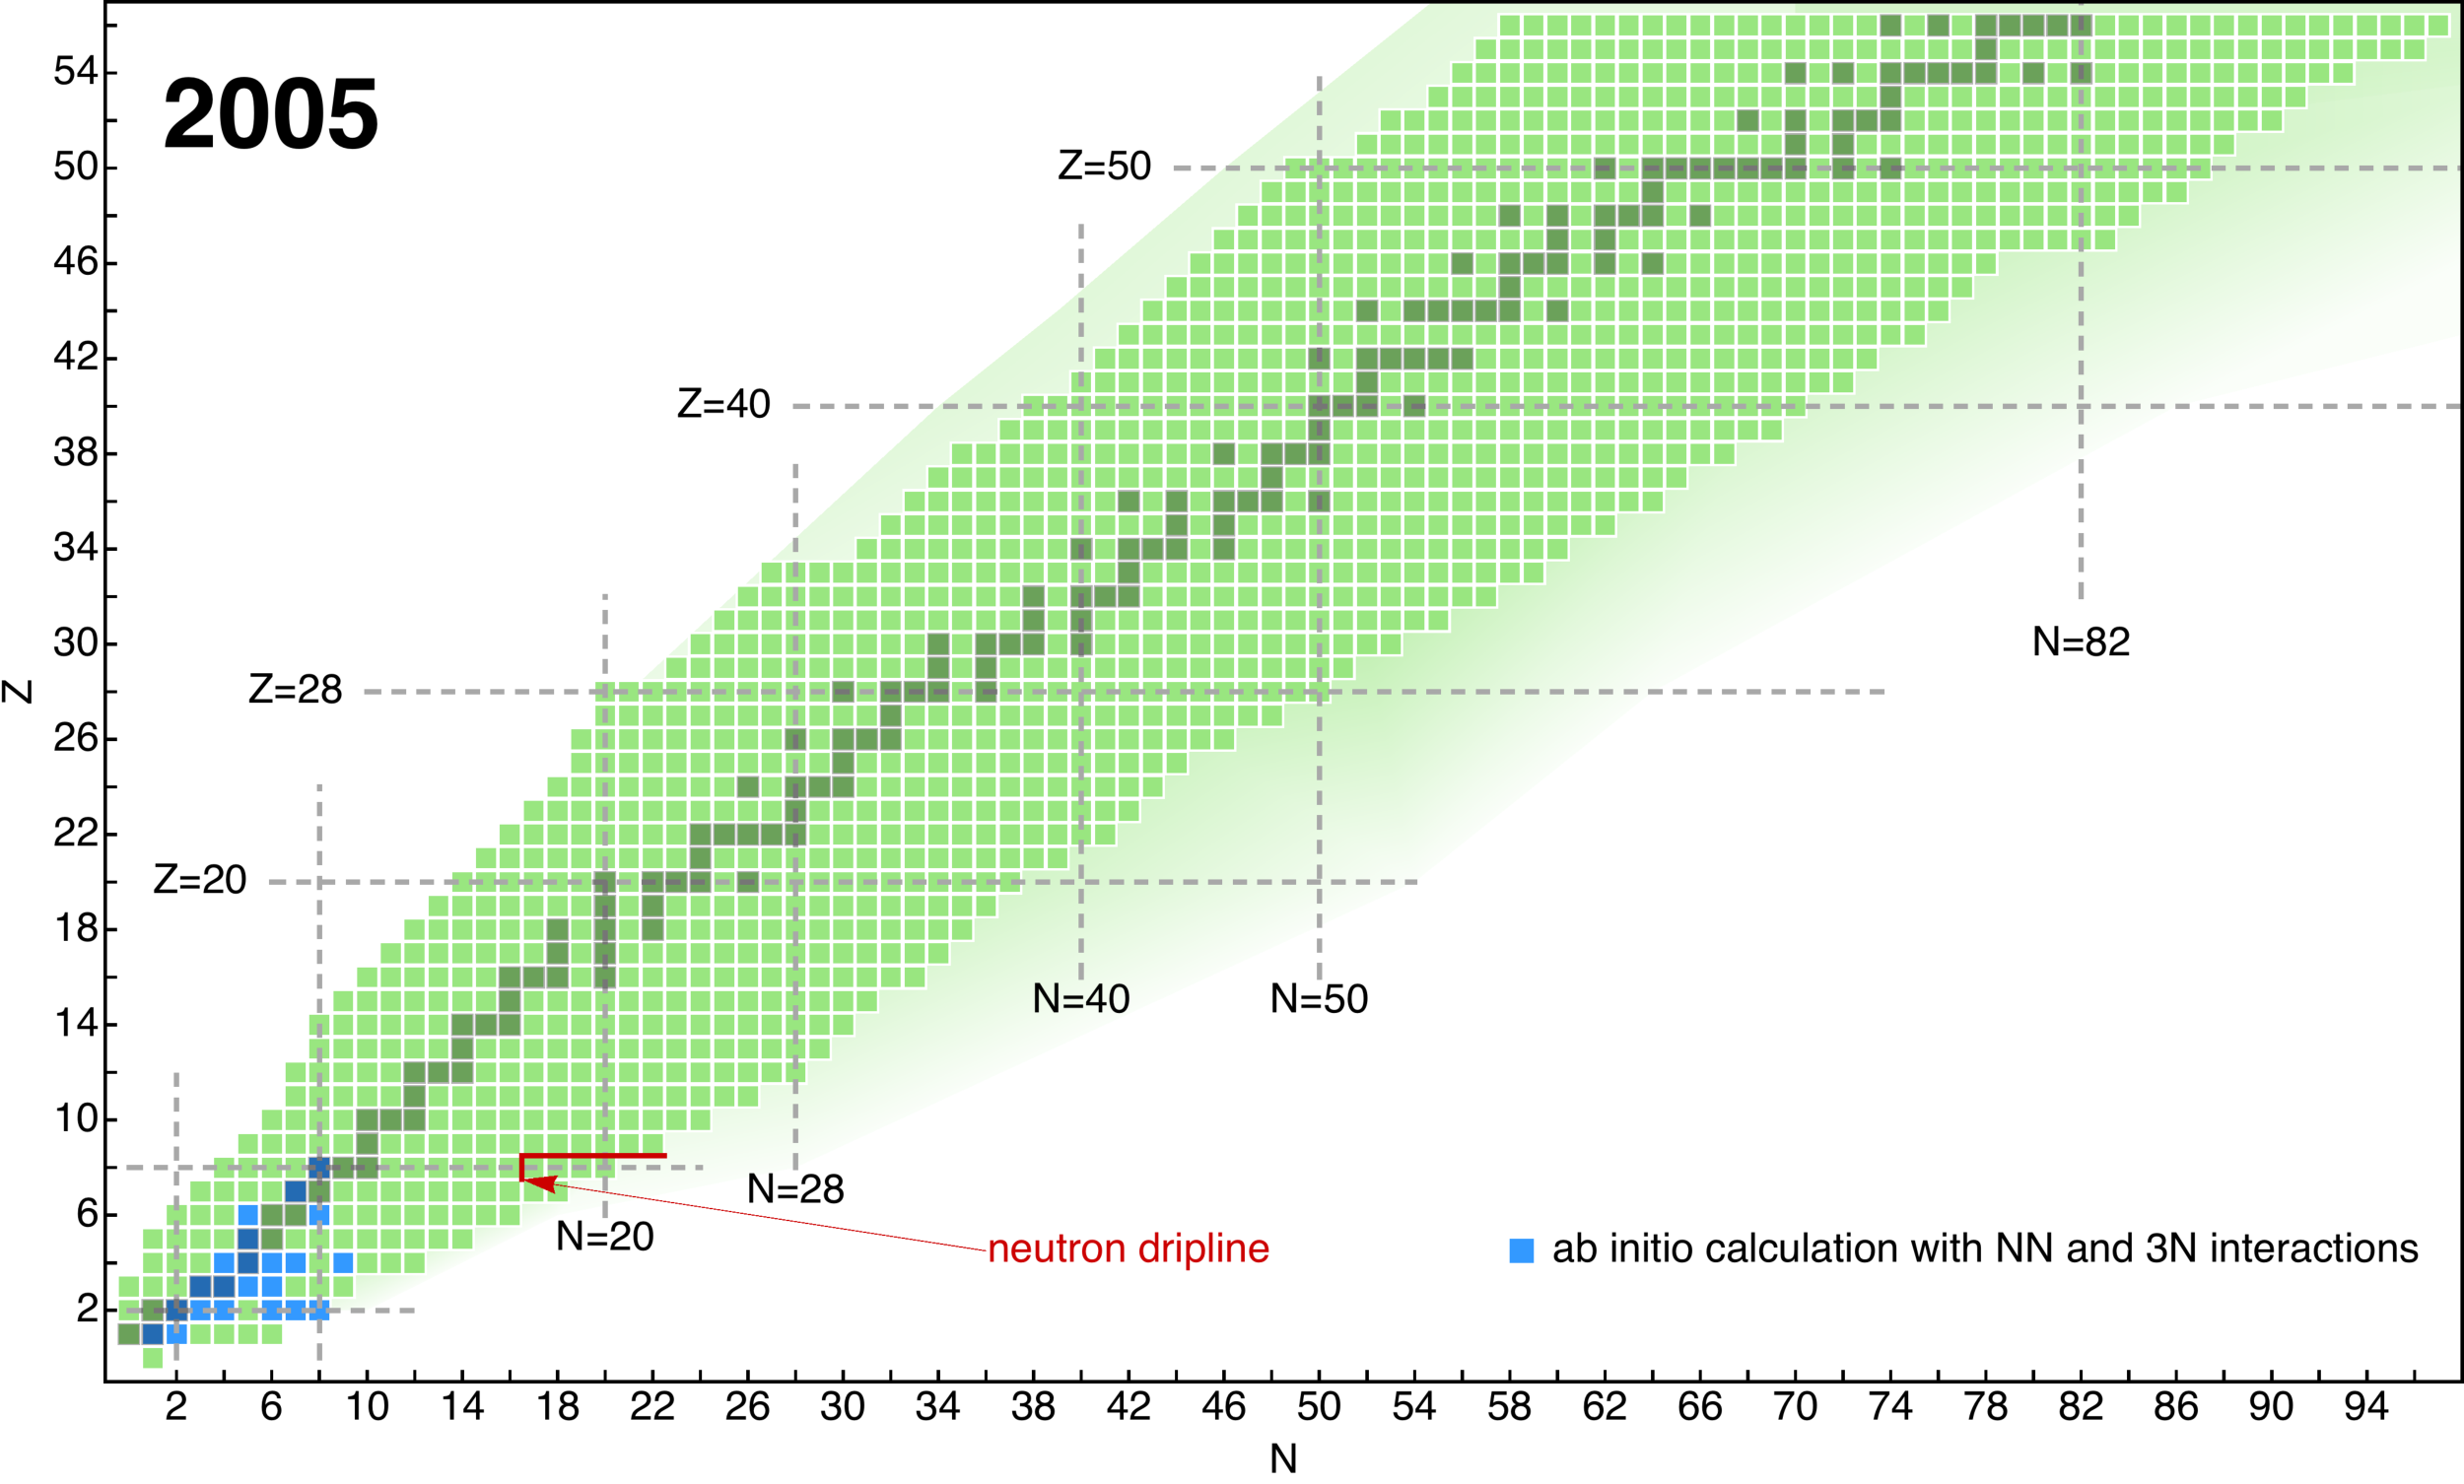
\includegraphics[width=0.80\textwidth]{introduction/ab-initio_nuclear_chart_2005.pdf}
  \end{subfigure}
  
  \begin{subfigure}{\textwidth}
    \centering
    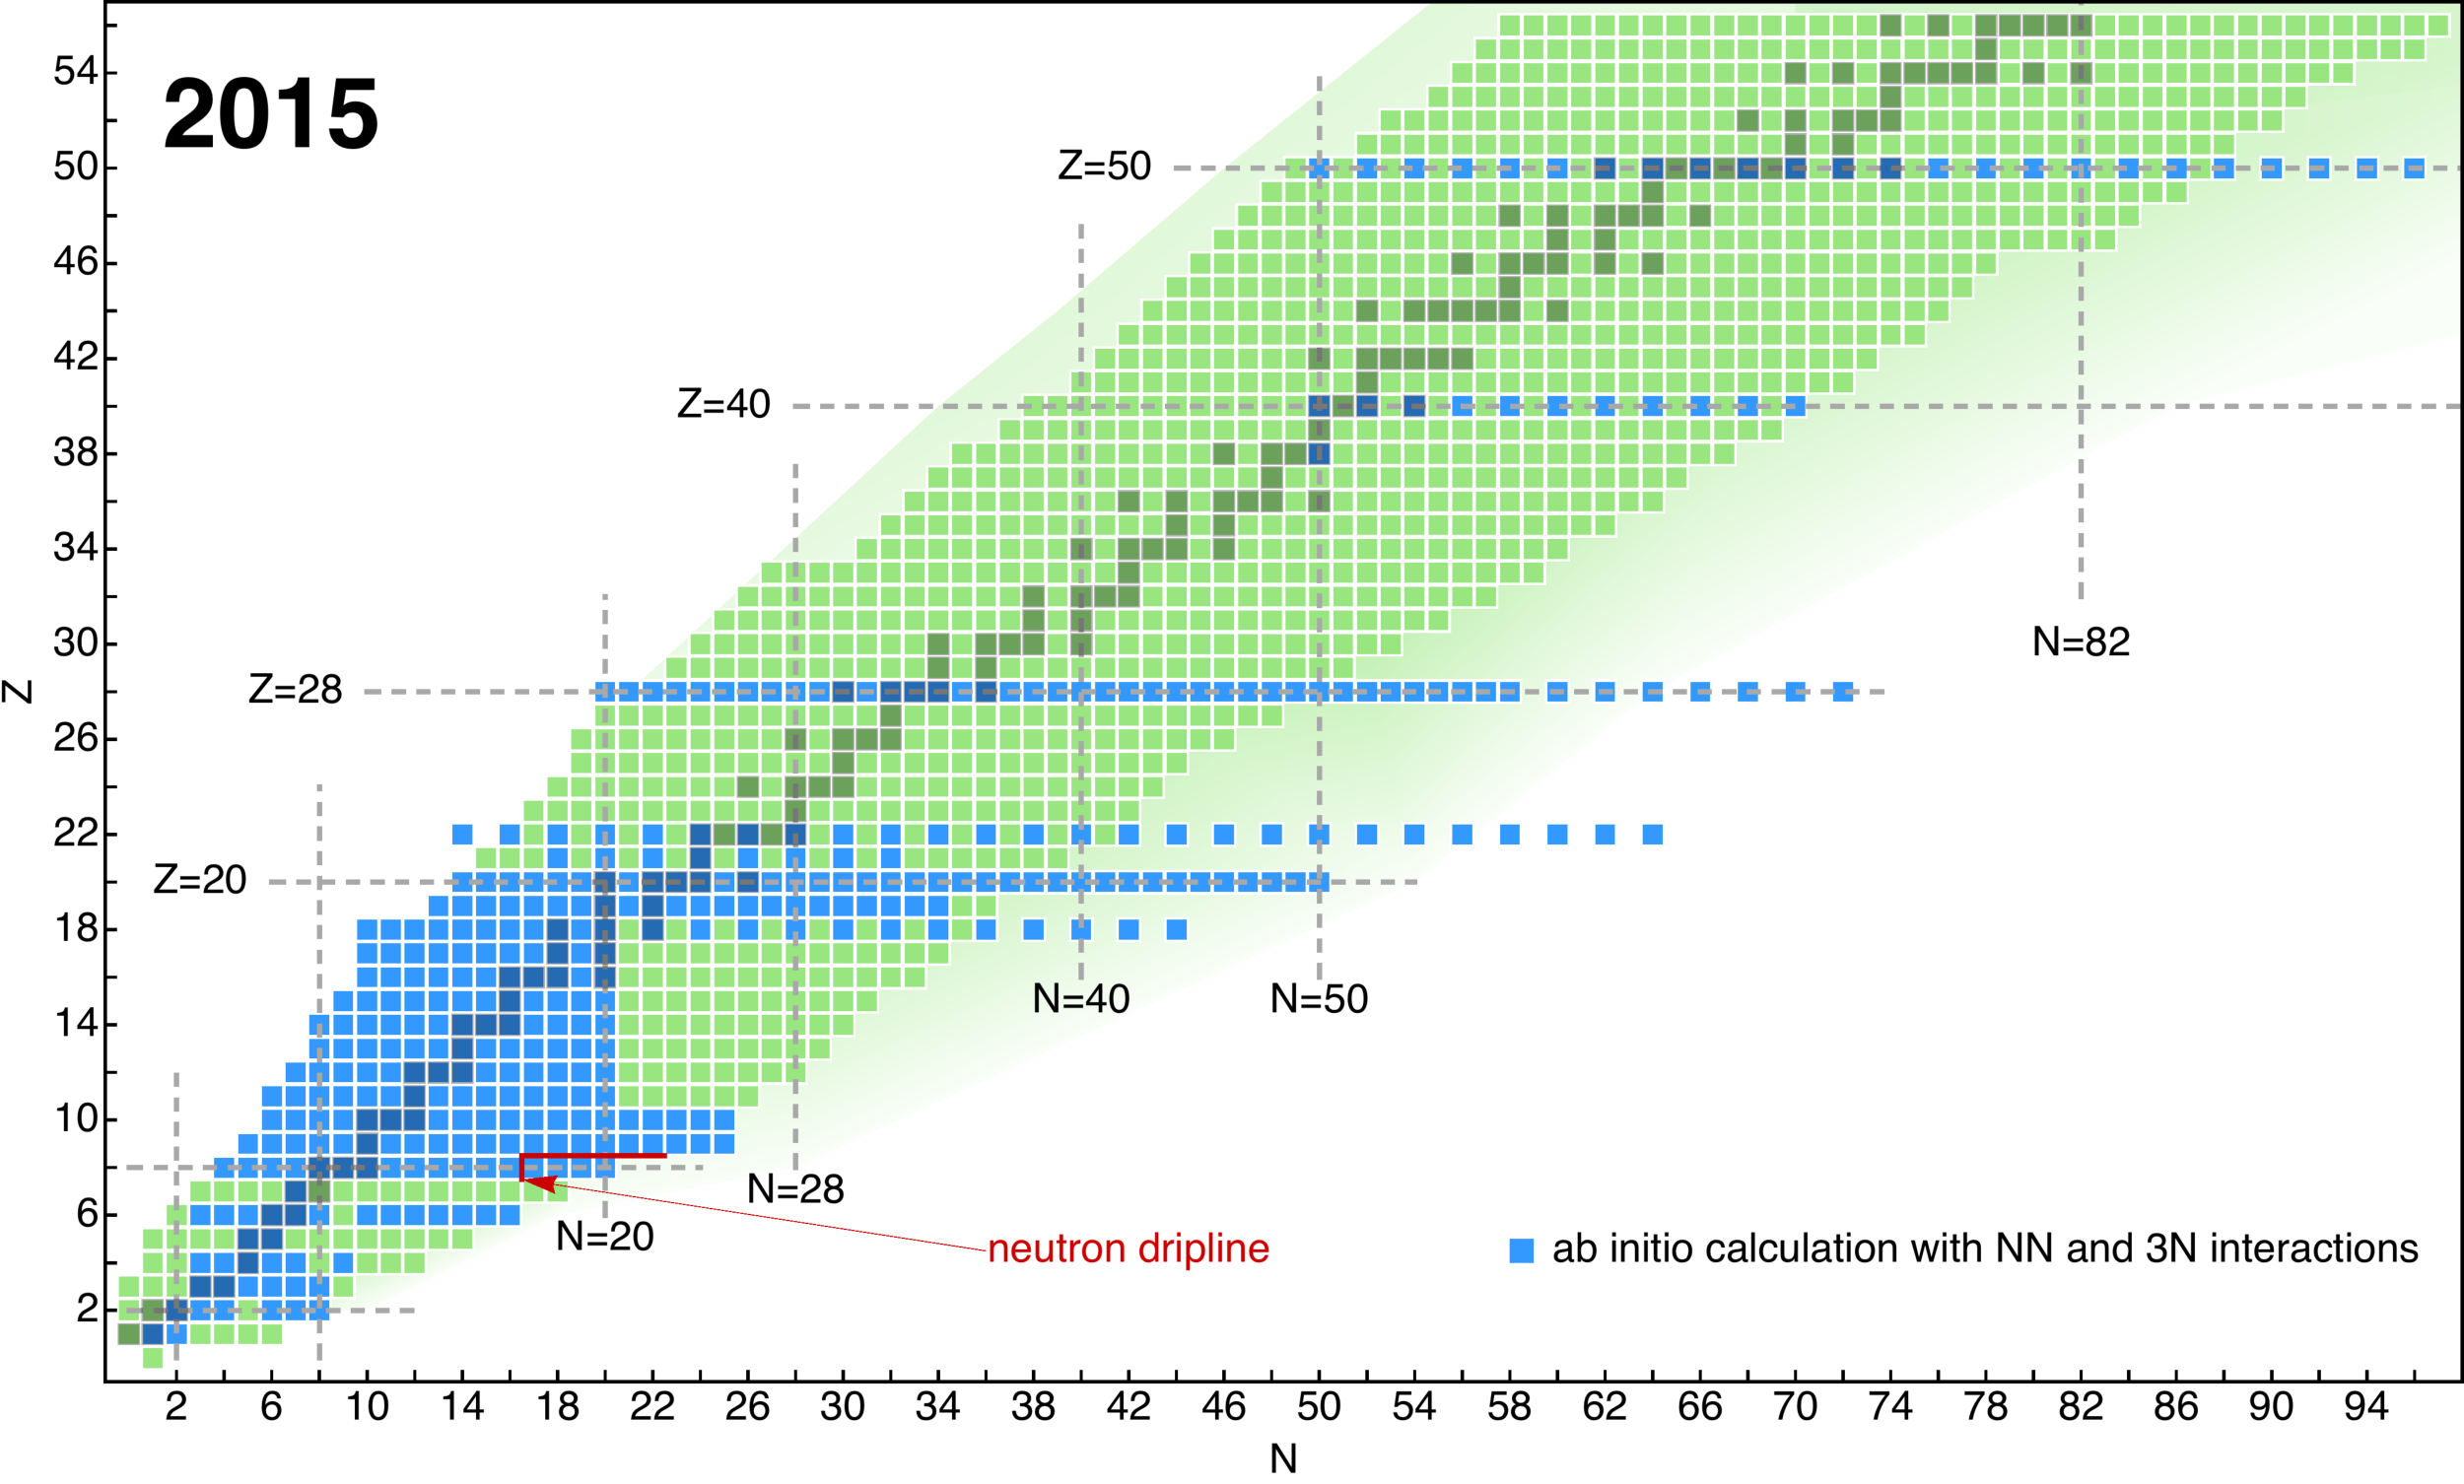
\includegraphics[width=0.80\textwidth]{introduction/ab-initio_nuclear_chart_2015.pdf}
  \end{subfigure}
  \caption{Nuclear Chart blah blah blah ab-initio}
  \label{fig:AbInitioChart}
\end{figure}

\begin{figure}
  \centering
  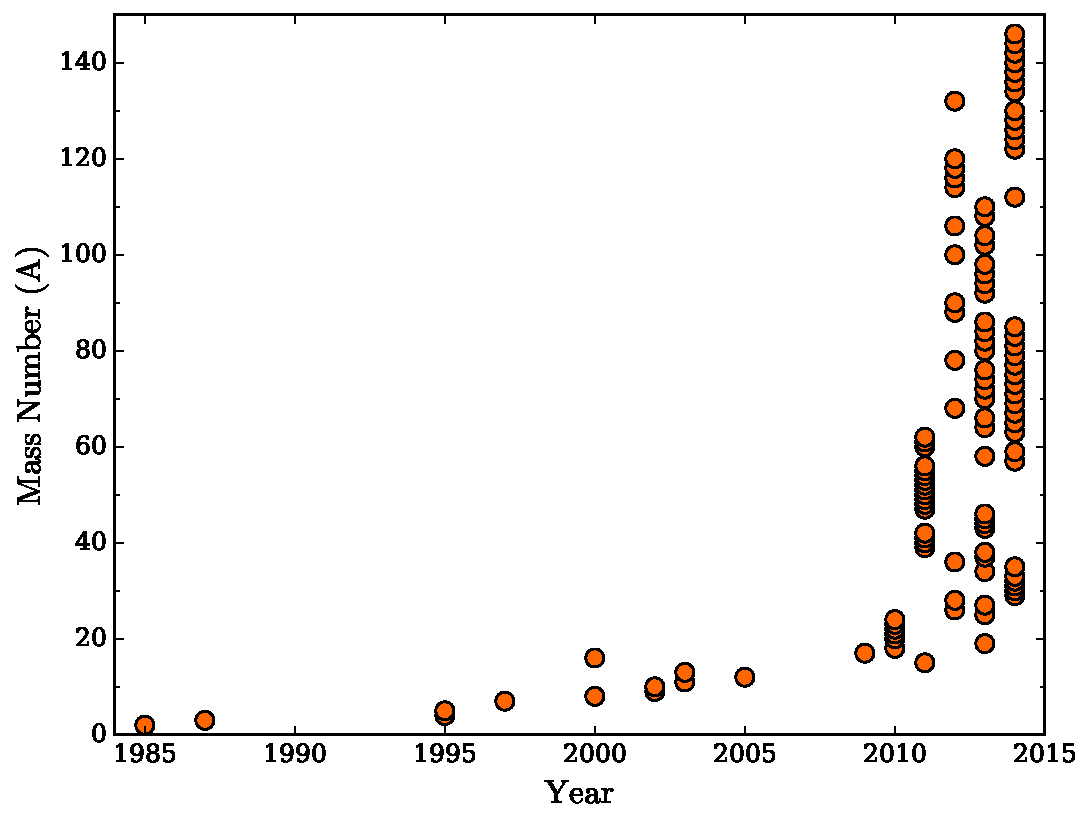
\includegraphics[width=0.80\textwidth]{introduction/ab-initio_progress.pdf}
  \caption{ab-initio progress blah blah blah}
  \label{fig:AbInitioProgress}
\end{figure}

\section{Ab-Initio Descriptions of Beta Decay}

\end{document}
